\chapter{Trace Assisted Caching}
\label{chap:trace-assisted-caching}

Having now considered the literature we move on to a theoretical explanation of the new technique this thesis proposes. We will start by exploring the motivation for this new technique; give a theoretical, processor agnostic, description of how to works; and follow that with a section that explains how this technique will bring benefit to hardware that implements this system.

\section{Motivation}

If we return to the central question of this thesis, we are trying to understand how memory latency can be reduced to reduce overall program runtime. However the results of the literature review in the previous chapter appear to show that we are blocked along all the avenues considered as a route to this goal. For example, cache policies definitely show some ability to reduce latency by making smarter decisions about which elements should be replaced and when that should happen. However there is an upper limit on their ability to reduce latency, namely the \texttt{OPT} ceiling, and much of this gap has been closed with the research we've seen. As a result more work in this area is going to follow the law of diminishing returns, leading a lot of researchers to abandon work on cache policies because they are 'good enough` \cite{podlipnigSurveyWebCache2003}. Moreover, \texttt{OPT} cannot be implemented because perfect clairvoyance is impossible in general and even if it could be the effectiveness of \texttt{OPT} is still not 100\%. So even if we could implement a version of \texttt{OPT} that worked there are serious questions as to whether we'd want to or whether there were more effective ways to reduce latency in other areas.

\subsection{Defining the Key Problems}

If we look at the other key areas of the literature we see the same story over and over again. Either the economics of the decision don't balance, i.e. we need a very large hardware budget to achieve a comparatively small drop in latency; or techniques don't have enough information available to them to make good decisions. So if we boil down these problems what is the root cause? I believe it stems from two key problems, the first is that these techniques are making decisions based upon limited information. In the case of caches for example, they can only react to information once a miss has happened, and the only option they have is to perform a costly memory access. With more information they could react earlier and have more scope to perform other actions, not just performing a memory access. Even with pre-fetching, which is more pro-active, the problem recurs. Simpler pre-fetch schemes like \gls{obl} or stride are similarly limited in the information they have, and even in more advanced schemes they lack the knowledge of dynamic information in the program, like effective addresses, to make very high quality decisions.

The second key problem is an assumption that is made on the part of computer architects is a belief in the synchronicity of the memory and computation parts of a computer. This leads to systems that exhibit limited potential for memory/computation parallelism because in their model of execution all instructions take the same amount of time to execute which is simply not the case. Some work, particularly in the realm of pre-fetching has tried to address this \cite{veidenbaumDecoupledAccessDRAM1997, vanderwielCompilerassistedDataPrefetch1999, mutluRunaheadExecutionAlternative2003}, by proposing systems whereby the memory system can work independently of the computation system. However even these papers do not go as far as they could in pursuing this independence because of the problem of a lack of information. In particular, if you cannot predict the effective addresses of memory accesses you are forced to incur lots of stalls in your memory execution, while you wait for non-obvious effective addresses to be calculated. This will increase the level of synchronicity between memory and computation which you are trying to avoid. Otherwise, you accept that you are predicting these memory accesses and have to allow for the fact that you may get that wrong and have to roll-back any changes made. 

\subsection{Tracing: A Solution}

These two problems together form the block that stops most of the techniques we've seen being more effective. A lack of information and the assumption of synchronicity place a restraint on the level of pre-emptive action that techniques can undertake. But how might these problems be solved? What if we assumed a certain level of asynchronicity between memory and computation systems? What information would we need to not hit the problems that previous approaches have? The key is access to the effective memory addresses before the memory operation has started. If this information were available it would be immediately obvious to a memory system when memory instructions could be re-ordered, because there would be no doubt as to whether two instructions referenced the same location in memory. It would also be possible to pre-fetch much more effectively because the pre-fetcher would know far ahead of time what data was required and could plan accordingly. 

So we know what data we need but how might we access it? A central objection comes to fore already, which says that information like effective addresses simply do not exist before they are required, so they are already available as early as they could be. Consequently we are going need some way to record these effective addresses, in an efficient way, and then make those recordings available to the processor as it progresses through the memory instructions present in the program. These `recordings' would be complete program traces, these would record the exact set of steps taken by the program through its execution and would consequently contain the vital link between instructions executed by the processor and the effective addresses they targeted. But this is only one part of what would be required, we will also need to add more intelligence to the L1 cache such that it can be responsible for querying these new traces and pro-actively responding to their contents if it's possible to do so. This would allow the cache and memory system to run-ahead of the processor, up to a point, executing high latency memory instructions much before they are required. This process is trace-assisted caching, using tracing to allow the cache to run-ahead of the processor to bring forwards memory operations, reducing run-time by increasing the overlap of high and low latency instructions.

\section{A Schematic Design}

Now we have seen a theoretical description of how trace assisted caching works let us consider a schematic design for the system. Chapter \ref{chap:experimental-design} will focus on the implementation but let us consider, at a conceptual level, the key pieces of an implementation and their function before being bogged down in the exact details of how a system like this is implemented. So first let us imagine a single-core \gls{cpu} with a Harvard Architecture, with an L1 data cache. This cache can be direct-mapped or set-associative and implements a replacement policy of some kind. This can be seen in the diagram below:

\begin{figure}
	\tikzstyle{block} = [draw, rectangle, text width=2cm, text centered, minimum height=1.2cm, node distance=2.7cm]
\tikzstyle{computation-block} = [block, fill=blue!30]
\tikzstyle{memory-block} = [block, fill=green!30]
\tikzstyle{cache-block} = [block, fill=orange!30]

\begin{center}
	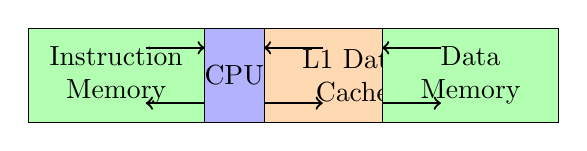
\begin{tikzpicture}
	
	 \node [computation-block] (CPU) {CPU};
	 \node [memory-block, left of=CPU] (Imem) {Instruction Memory};
	 \node [cache-block, right of=CPU] (DCache) {L1 Data Cache};
	 \node [memory-block, right of=DCache] (Dmem) {Data Memory};
	
	\draw [thick] [->] ([yshift=1em]DCache.east)-- ([yshift=1em]Dmem.west);
	\draw [thick] [<-] ([yshift=-1em]DCache.east)-- ([yshift=-1em]Dmem.west);

	\draw [thick] [->] ([yshift=1em]CPU.east)-- ([yshift=1em]DCache.west);
	\draw [thick] [<-] ([yshift=-1em]CPU.east)-- ([yshift=-1em]DCache.west);
	
	\draw [thick] [->] ([yshift=1em]CPU.west)-- ([yshift=1em]Imem.east);
	\draw [thick] [<-] ([yshift=-1em]CPU.west)-- ([yshift=-1em]Imem.east);
	
	\end{tikzpicture}
\end{center}
	\caption[Basic Processor Architecture]{The basic design begins with a processor with a Harvard Architecture. This is so that the effect of any caching on the data side can be isolated and quantified more easily.}
\end{figure}

As was alluded to in the previous section there are two key pieces that form the architecture for Trace Assisted Caching: the trace recorder and the intelligent cache. Each will be described in turn. We'll also describe any changes that would need to be made to the processor to support these new pieces of hardware.

\subsection{Trace Recorder}

The trace recorder would sit attached to the processor and would monitor the internal control signals emitted by the processor. These control signals would not only be those that manipulated memory but would initially be every pipeline phase of every instruction the processor executed. This would require changes to the processor, exposing previously enclosed signals, but because we have to perform this recording asynchronously from the processor, so as not to block its execution unnecessarily, this is the only option available to us.

\begin{figure}
	\tikzstyle{block} = [draw, rectangle, text width=2cm, text centered, minimum height=1.2cm, node distance=1.5cm and 1cm]
\tikzstyle{computation-block} = [block, fill=blue!30]
\tikzstyle{memory-block} = [block, fill=green!30]
\tikzstyle{cache-block} = [block, fill=orange!30]
\tikzstyle{tac-block} = [block, fill=red!30]

\begin{center}
	\begin{tikzpicture}
	
	 \node [computation-block] (CPU) {CPU};
	 \node [memory-block, left=of CPU] (Imem) {Instruction Memory};
	 \node [tac-block, above=of CPU] (TRecord) {Trace Recorder};
	 \node [tac-block, right=of TRecord] (TRepo) {Trace Repository};
	 \node [memory-block, right=of CPU] (Dmem) {Data Memory};
	
	\draw [thick] [->] ([yshift=1em]CPU.east)-- ([yshift=1em]Dmem.west);
	\draw [thick] [->] ([yshift=1em, xshift=1em]CPU.east) |- ($(TRecord.south) - (0,5mm)$) -| (TRecord.south);
	\draw [thick] [<-] ([yshift=-1em]CPU.east)-- ([yshift=-1em]Dmem.west);
	
	\draw [thick] [->] ([yshift=1em]CPU.west)-- ([yshift=1em]Imem.east);
	\draw [thick] [->] ([yshift=1em, xshift=-1em]CPU.west) |- ([yshift=1em]TRecord.west);
	\draw [thick] [<-] ([yshift=-1em]CPU.west)-- ([yshift=-1em]Imem.east);
	
	\draw [thick] [->] (TRecord.east) -- (TRepo.west);
	
	\end{tikzpicture}
\end{center}
	\caption[Basic Architecture with Trace Recorder]{The trace recorder takes in information from both the instruction stream and the data stream to produce a stream of pipeline stages bundled into instructions. This is stored in the trace repository after filtering to remove all non-memory instructions.}
\end{figure}

The amount of data a trace like this would generate is potentially gargantuan, multiplying the amount which already exists in instruction traces by the length of the pipeline, but there are several reasons why this level of detail is required. The first is that the goal of this recording is to link together instructions in the program with effective addresses they generate. If you record at a more granular level, it can be very difficult to associate memory accesses with the instructions that generated them. Recording at the level of pipeline stages and aggregating to instructions later means there is no ambiguity. This does also mean that we have to take into account branching behaviour and stalls in our recorder, and this will be explored further in Chapter \ref{chap:experimental-design}, but this would give us a complete trace, at the level of pipeline stages, for any program that runs on the processor. In addition tracing at the level of pipeline stages means that you are recording a serialised data stream, meaning there is no need to do any de-multiplexing or complex analysis to associate actions with instructions, at the level of pipeline stages there can only be one instruction per stage at a time. 

Now we have this potentially gargantuan amount of data we have to filter it down in some way. Even for a small processor running a short program this could lead to gigabytes of data being generated and this is simply not viable to store or query. The first thing we can do is to throw away the details of each individual pipeline stage, these are not needed to instruct the memory system directly, we simply use them as a way to ensure the correct ordering of the memory instructions. The second piece of filtering is to remove any instructions that do not have memory implications, this could be as much as 60\% of the instructions captured. By filtering and aggregating using these two criteria we can produce a trace that is an ordered list of instructions linked to effective memory addresses. An example of which is shown below:

\begin{figure}
	\tikzset{
	print/.style={ % requires library shapes.symbols
		draw,
		tape,
		tape bend top=none
	}
}

\begin{tikzpicture}

	{
		\renewcommand*\thelstnumber{\ifnum\value{lstnumber}<8 0\fi \xintDecToHex{\the\value{lstnumber}*4}}
		
		\node [print, fill=yellow!30] (assembly-code) {
			\begin{minipage}{.48\textwidth}
				\lstset{
				language=risc-v, 
				basicstyle=\ttfamily, 
				numbers=left,  
				numberstyle=\ttfamily,
				firstnumber=149,
				aboveskip=0pt,belowskip=0pt
				}
				\lstinputlisting[lastline=1, stepnumber=2]{diagrams/trace_assisted_caching/fac_excerpt.S}
				\lstinputlisting[firstline=2,lastline=2,backgroundcolor=\color{red!60}, firstnumber=150]{diagrams/trace_assisted_caching/fac_excerpt.S}
				\lstinputlisting[firstline=3,lastline=3,backgroundcolor=\color{blue!50}, stepnumber=2]{diagrams/trace_assisted_caching/fac_excerpt.S}
				\lstinputlisting[firstline=4, lastline=4, firstnumber=152]{diagrams/trace_assisted_caching/fac_excerpt.S}
				\lstinputlisting[firstline=5,lastline=5,backgroundcolor=\color{olive!50}, stepnumber=2]{diagrams/trace_assisted_caching/fac_excerpt.S}
				\lstinputlisting[firstline=6, lastline=6, firstnumber=154]{diagrams/trace_assisted_caching/fac_excerpt.S}
				\lstinputlisting[firstline=7,lastline=7,backgroundcolor=\color{violet!50}, stepnumber=2]{diagrams/trace_assisted_caching/fac_excerpt.S}
				\lstinputlisting[firstline=8,lastline=8,backgroundcolor=\color{brown!50},firstnumber=156]{diagrams/trace_assisted_caching/fac_excerpt.S}
				\lstinputlisting[firstline=9, lastline=9, stepnumber=2]{diagrams/trace_assisted_caching/fac_excerpt.S}
				\lstinputlisting[firstline=10,lastline=10,backgroundcolor=\color{pink!50},firstnumber=158]{diagrams/trace_assisted_caching/fac_excerpt.S}
				\lstinputlisting[firstline=11,lastline=18, stepnumber=2, ,firstnumber=159]{diagrams/trace_assisted_caching/fac_excerpt.S}
				\lstinputlisting[firstline=19, lastline=19, backgroundcolor=\color{orange!50},stepnumber=2]{diagrams/trace_assisted_caching/fac_excerpt.S}
				\lstinputlisting[firstline=20, lastline=20, backgroundcolor=\color{teal!50}, firstnumber=168]{diagrams/trace_assisted_caching/fac_excerpt.S}
				\lstinputlisting[firstline=21, stepnumber=2, firstnumber=169]{diagrams/trace_assisted_caching/fac_excerpt.S}
			\end{minipage}
			};
	}
	\node [right= of assembly-code] (trace) {
		\pgfplotstabletypeset[
			col sep=comma, 
			columns={Effective Address, Instruction}, 
			columns/Effective Address/.style={column type={|c|},string type},
			columns/Instruction/.style={column type={c|},string type},
			every head row/.style={after row=\hline, before row=\hline},
			every last row/.style={after row=\hline},
			assign column name/.style={/pgfplots/table/column name={\textbf{#1}}},
			every row no 0/.style={before row={\rowcolor{red!50}}},
			every row no 1/.style={before row={\rowcolor{blue!50}}},
			every row no 2/.style={before row={\rowcolor{olive!50}}},
			every row no 3/.style={before row={\rowcolor{violet!50}}},
			every row no 4/.style={before row={\rowcolor{brown!50}}},
			every row no 5/.style={before row={\rowcolor{orange!50}}},
			every row no 6/.style={before row={\rowcolor{teal!50}}},
			every row no 7/.style={before row={\rowcolor{pink!50}}}
		] {diagrams/trace_assisted_caching/trace.csv}
	};
	
	
\end{tikzpicture}
	\caption[Program Fragment with Trace]{On the left can be seen a fragment of the disassembled version of the benchmark \texttt{fac.c} which is part of the Mälardalen Benchmark Suite \cite{gustafssonMalardalenWCETBenchmarks2010}. On the right can be seen the trace that relates to this part of the file, with effective addresses next to each memory instruction. The colours indicate which trace element maps to each instruction in the disassembled file and it can be seen that the trace follows the execution of the program, following jumps and branches as they arise.}
\end{figure}


We now need to turn our attention to a second problem which is how should this be stored? We cannot use up data memory for this because it could affect the retrieval of actual program data, so we need a separate memory store to keep these traces accessible to the intelligent cache. This takes the form of a trace repository that is stored in memory so it can be queried by the cache on each clock cycle when the program is run for a second time. It's also possible to seed this trace repository with data from a previous run if you didn't want to have to run the program once in a `training phase'. Issues such as where this repository is to be stored, how it might be fetched from efficiently and how it might be built up iteratively over multiple runs will be dealt with in future sections. 

So if we consider an execution of a program on a processor that is architected this way. The program would execute as normal, though the cache itself would by bypassed during the recording phase, this is so that we are recording the `worst case' behaviour, rather than that caused by the cache. While the \gls{cpu} executes the control signals it generates are tracked and recorded by the trace recorder. Filtered as the recording occurs and sent to the trace repository. Once the program reaches its end, as marked by it entering the processor's trap state, the trace recorder will stop recording and the data will held in the repository is then available for the second and further runs of the program.

\subsection{Intelligent Cache \& Memory System}

Now that we have a highly filtered version of the trace stored we can start to use it to allow the cache and memory system to work asynchronously from the processor. This works in the following way: on every clock cycle instead of sitting waiting for the processor to issue a command to it the cache polls the trace repository. The trace repository then returns to the cache the next trace in the stream that it had recorded in the previous run of the program. Now the cache has potentially two requests it could service, a pre-emptive request or an on demand request. In all cases the on-demand request would take priority because we don't want to introduce further latency by delaying a request from the processor. An in an ideal world the pre-emptive request will be sufficiently far ahead of the on-demand request that delaying it will not cause further latency. 

If there is no on-demand request the cache seeks to service the pre-emptive and there are four scenarios that could occur, depending on the content of the instruction to be executed:

\begin{enumerate}[label=\textbf{Scenario \arabic*:}, align=left, leftmargin=*,labelindent=16pt]
	\item If the pre-emptive instruction is a load and there is space within the cache then simply execute the instruction.
	\item If the pre-emptive instruction is a store and there is space in the cache then you cannot execute it because you don't know what data is to be stored there. However you can reserve the space in the cache to make sure it isn't overwritten by another action.
	\item If it's a load but there is no space in the cache then perform a write-back and then do the same as in Scenario 1.
	\item If it's a store and there's no space again perform the write-back and then reserve the space.
\end{enumerate}

These 4 scenarios are illustrated in Figure \ref{fig:scenarios}

\tikzstyle{cell} = [rectangle,draw=black, fill=green!30]
\tikzstyle{space} = [minimum height=1.5em,matrix of nodes,row sep=-\pgflinewidth,column sep=-\pgflinewidth,text depth=0.5ex,text height=2ex,nodes in empty cells]

\begin{figure}[htbp]
	\begin{center}
		\begin{subfigure}[b]{\textwidth}
			\begin{center}
				\begin{tikzpicture}
     	\node [rectangle, draw, fill=blue!30, minimum height=2cm] (trace-repo) {Trace Repository};
     	\node [rectangle, draw, fill=blue!30, left=of trace-repo, label=below:{Latest Trace Entry}] (tr-output) {\texttt{fe442783}, \texttt{fee4}};
		\matrix [
			left=of tr-output, space, 
			column 1/.style={minimum width=3em,nodes={cell,minimum width=2em}},
			column 2/.style={minimum width=3em,nodes={cell,minimum width=2em}},
			column 3/.style={nodes={cell,minimum width=6em}}
			] 
		(cache)
		{
			\textbf{R} & \textbf{O} & \textbf{D} \\
			0  & 1 & \texttt{0x12345678} \\   
			0  & \textbf{1} & \textbf{\texttt{0xFFEEDDCC}} \\   
			0  & 1 & \texttt{0xFEDCBA98} \\   
		};
		\node [rectangle, draw, fill=green!30, below= of cache, minimum width=5cm] (main-memory) {Main Memory};
		\node [above= of cache-1-2, xshift=2em, yshift=-2em] {\textbf{Cache}};
     	
     	\draw [thick] [->] (trace-repo.west) -- (tr-output.east);
     	\draw [thick] [->] (tr-output.west) -- (cache.east);
     	\draw [thick] [->] ([xshift=-1em]cache.south) -- ([xshift=-1em]main-memory.north) node[midway, left] {\textbf{\texttt{0xFEE4}}};
     	\draw [thick] [->] ([xshift=1em]main-memory.north) -- ([xshift=1em]cache.south) node[midway, right] {\textbf{\texttt{0xFFEEDDCC}}};
\end{tikzpicture}
				\caption{Scenario 1 - A load where the cache has capacity, the load is simply executed by the cache and stored in the correct location.}
			\end{center}
		\end{subfigure}
		\begin{subfigure}[b]{\textwidth}
			\begin{center}
				\begin{tikzpicture}
    \node [rectangle, draw, fill=blue!30, minimum height=2cm] (trace-repo) {Trace Repository};
    \node [rectangle, draw, fill=blue!30, left=of trace-repo, label=below:{Latest Trace Entry}] (tr-output) {\texttt{fe042423}, \texttt{fee8}};
    \matrix [
    left=of tr-output, space, 
    column 1/.style={minimum width=3em,nodes={cell,minimum width=2em}},
    column 2/.style={minimum width=3em,nodes={cell,minimum width=2em}},
    column 3/.style={nodes={cell,minimum width=3.5em}}
    ] 
    (cache)
    {
		     	0  & 1 & \texttt{0x12345678} \\   
		     	\textbf{1} & 0 & \texttt{0x00000000} \\   
		     	0  & 1 & \texttt{0xFEDCBA98} \\   
    };
    \node [yshift=-2em, above= of cache-1-1] {R};
    \node [yshift=-2em, above= of cache-1-2] {O};
    \node [yshift=-2em, above= of cache-1-3] {D};
    \node [rectangle, draw, fill=green!30, below= of cache, minimum width=5cm] (main-memory) {Main Memory};
    
    \draw [thick] [->] (trace-repo.west) -- (tr-output.east);
    \draw [thick] [->] (tr-output.west) -- (cache.east);
    \draw [thick] [->] ([xshift=-1em]cache.south) -- ([xshift=-1em]main-memory.north);
    \draw [thick] [->] ([xshift=1em]main-memory.north) -- ([xshift=1em]cache.south);
\end{tikzpicture}
				\caption{Scenario 2 - A store where the cache has capacity, the store cannot be actioned because the data to store is not known in advance but the cache element is reserved.}
			\end{center}
		\end{subfigure}
		\begin{subfigure}[b]{\textwidth}
			\begin{center}
				\input{diagrams/trace_assisted_caching/scenario_3.tex}
				\caption{Scenario 3 - If the cache doesn't have capacity for a load then perform the write-back to memory first and then act in accordance with Scenario 1}
			\end{center}
		\end{subfigure}
	\caption[Illustration of Pre-emptive Scenarios]{Illustrations of the four scenarios described. The R, O and D columns above the cache in each diagram stand for Reserved, Occupied and Data respectively. The bold text indicates elements that change throughout the scenario. The cache may also have other elements, such as validity bits, but these are omitted for the sake of clarity and are mostly implementation details. Scenario 4 is printed on the next page}
	\label{fig:scenarios}
	\end{center}
\end{figure}
\begin{figure}\ContinuedFloat
	\begin{center}
    	\begin{subfigure}[b]{\textwidth}
    		\begin{center}
    			\input{diagrams/trace_assisted_caching/scenario_4.tex}
    			\caption{Scenario 4 - If the cache doesn't have capacity for a store then again perform a write-back and proceed as Scenario 2}
    		\end{center}
    	\end{subfigure}
	\end{center}
\end{figure}

All this means that when the processor catches up to the pre-emptive action it will either, have the data already in the case of scenario 1 or 3 or will be guaranteed to not have to perform a write-back in the case of scenario's 2 or 4. As a result latency will decrease because all these operations will have been done ahead of time. 

There are some limitations to this approach of course, most of which relate to how far ahead of the processor the memory system can go. For one thing no attempt is made to re-order the memory operations in the way that an \gls{ooo} processor would. This is mostly to simplify the implementation and to avoid the complex problems of ensuring consistency over multiple interleavings of the instructions. As a result of this there are situations where no more pre-emptive actions can be taken until the processor has performed some critical action. For example should a processor issue pre-emptive instructions such that it tries to perform a \texttt{LOAD} to a location that is being reserved for a \texttt{STORE} then it will not take any action until the processor has completed the \texttt{STORE} because it cannot know in advance what data will be part of the \texttt{STORE} operation. This is shown in Figure \ref{fig:problem-scenario}. In this situation the processor will keep polling to discover if the operation has happened and can then act accordingly. There is a potential for future work to consider continuing to execute independent instructions at this point but that was not considered in this work. 

\begin{figure} [htbp]
	\begin{center}
		\input{diagrams/trace_assisted_caching/problem_scenario.tex}
		\caption[Illustration of a Block on Pre-emptive Actions]{In this situation the latest trace entry is attempting a \texttt{LOAD} into a location that is reserved for a store. At this point the pre-emptive execution cannot continue because the \texttt{STORE} has not yet happened. The only option is for the pre-emptive instruction to poll the cache until the \texttt{STORE} has happened and then processing can continue.}
		\label{fig:problem-scenario}
	\end{center}
\end{figure}

A final point to address is that this scheme is agnostic to the details of the cache that is in the underlying hardware. In this thesis both an 8-way associative and a direct-mapped cache were used but there is nothing special about these choices. It would be very easy to implement higher associativity caches or larger caches with very few changes to the trace-assisted mechanism. This also brings up the possibility of varying the replacement policy for the cache to see if that, working in concert with this system had any benefit but again that was not considered in this work. 

This is trace assisted caching, recording the traces of programs, filtering them and then allowing the cache to run-ahead of the processor, leveraging the trace information to pre-emptively perform memory operations. But how do we know this is going to be a success? And how do we know that we're not going to introduce performance regressions from this technique? The next section answers these questions.

\section{Justification of Success}

Now we understand how trace assisted caching works at a high level we need to dig a little deeper into how we expect to benefit from this system. It's potentially a high investment in extra hardware, as a trace recorder is required as well as the changes to the cache and the trace repository, so there needs to be a commensurate benefit in runtime reduction to justify the expense. The best way to explain where the benefit derives from is by example and this explained below.

\subsection{Performance Increase}

Let us imagine a processor with a 4-stage pipeline, namely Fetch (IF), Decode (ID), Execute (EX) and Write-back (WB). Let us further suppose that there are no data forwarding mechanisms and for the sake of argument let us assume that fetches from main memory take 5 clock cycles from the submission of the request to the data being available. Now if that processor is executing the listing fragment below:

\lstinputlisting[label={listing:pipeline-test},language=risc-v, style=printing, caption={This code simply checks a loop condition based on some previous computations, a very common pattern.}, captionpos=b]{diagrams/trace_assisted_caching/justification.S}

Then we can consider what the pipeline might look like at each clock cycle, this can be seen in Figure \ref{fig:pipeline} starting from the execution of the \texttt{ADDI} line.

\begin{sidewaysfigure}
	\begin{center}
		\begin{tabular}{|*{15}{c|}}
	\hline
	\textbf{Instruction} & \multicolumn{14}{c|}{\textbf{Pipeline Stage}} \\
	\hline
	\texttt{ADDI} & \texttt{IF} & \texttt{ID} & \texttt{EX} & \texttt{WB} & & & & & & & & & & 	\\
	\texttt{ADD} & & \texttt{IF} & \texttt{ID} & \texttt{EX} & \texttt{WB} & & & & & & & & & 	\\
	\texttt{LW} & & & \texttt{IF} & \texttt{ID} & \texttt{EX} & \texttt{EX} & \texttt{EX} & \texttt{EX} & \texttt{EX} & \texttt{WB} & & & & \\
	\texttt{MUL} & & & & \texttt{IF} & \texttt{ID} & {\color{red}\texttt{STALL}} & {\color{red}\texttt{STALL}} & {\color{red}\texttt{STALL}} & {\color{red}\texttt{STALL}} & {\color{red}\texttt{STALL}} & \texttt{EX} & \texttt{WB} & & \\
	\texttt{MV} & & & & & \texttt{IF} & {\color{red}\texttt{STALL}} & {\color{red}\texttt{STALL}} & {\color{red}\texttt{STALL}} & {\color{red}\texttt{STALL}} & {\color{red}\texttt{STALL}} & \texttt{ID} & {\color{red}\texttt{STALL}} & \texttt{EX} & \texttt{WB} \\
	\hline
	\hline
	\textbf{Clock Cycle} & 0 & 1 & 2 & 3 & 4 & 5 & 6 & 7 & 8 & 9 & 10 & 11 & 12 & 13 \\ 
	\hline
	\hline
	\textbf{Memory System} & & & & & \texttt{PR} & \texttt{PR} & \texttt{PR} & \texttt{PR} & \texttt{AV} &&&&& \\
	\hline
\end{tabular}
		\caption[Pipeline Diagram - No Trace Assisted Caching]{The pipeline execution continues as normal until clock cycle 4 where the \texttt{LW} instruction enters its Execution phase. Because loading a value from main memory takes 5 clock cycles this extra latency is added not only to the \texttt{LW} but also to the \texttt{MUL} and \texttt{MV} instructions. Overall this leads to a program runtime of 14 clock cycles when the optimal time, assuming no pipeline stalls would be 8.}
		\label{fig:pipeline}
	\end{center}
\end{sidewaysfigure}

We see in this diagram that the pipeline fills up to its maximum depth but then as soon as the load instruction reaches the \texttt{EX} phase the pipeline is forced to stall while the memory access is dealt with, not only adding latency to its own execution but also to all the other instructions blocked behind it. Using trace assisted caching however we enter into a new situation as in Figure \ref{fig:ideal-pipeline}.

\begin{figure}
	\begin{center}
		\begin{tabular}{|*{11}{c|}}
	\hline
	\textbf{Instruction} & \multicolumn{10}{c|}{\textbf{Pipeline Stage}} \\
	\hline
	\texttt{ADDI} & \texttt{IF} & \texttt{ID} & \texttt{EX} & \texttt{WB} & & & & & & 	\\
	\texttt{ADD} & & \texttt{IF} & \texttt{ID} & \texttt{EX} & \texttt{WB} & & & & &	\\
	\texttt{LW} & & & \texttt{IF} & \texttt{ID} & \texttt{EX} & \texttt{WB} & & & &		\\
	\texttt{MUL} & & & & \texttt{IF} & \texttt{ID} & {\color{red}\texttt{STALL}} & \texttt{EX} & \texttt{WB} & &  \\
	\texttt{MV} & & & &  & \texttt{IF} & \texttt{ID} & {\color{red}\texttt{STALL}} & {\color{red}\texttt{STALL}} & \texttt{EX} & \texttt{WB} \\

	\hline
	\hline
	\textbf{Clock Cycle} & 0 & 1 & 2 & 3 & 4 & 5 & 6 & 7 & 8 & 9 \\ 
	\hline
	\hline
	\textbf{Memory System} & \texttt{PR} & \texttt{PR} & \texttt{PR} & \texttt{PR} & \texttt{AV} & & & & & \\
	\hline
\end{tabular}
		\caption[Pipeline Diagram - With Trace Assisted Caching]{In this example we see the power of trace assisted caching. If we assume the pre-emptive action to take is the one at line 3 in Listing \ref{listing:pipeline-test} then because the effective address can be known at clock cycle 0 the memory system can begin this load much earlier. As a consequence, the stalls associated with performing the memory operation are eliminated from the program's runtime reducing the overall runtime by 4 clock cycles. A decrease of nearly 30\%.}
		\label{fig:ideal-pipeline}
	\end{center}
\end{figure}


So we can see that because the processor has access to the effective address much earlier the cache miss can be pre-empted by the cache and dealt with much earlier. So when the processor actually executes the instruction the cache already has the data it requires and the latency is reduced by 10 cycles for the whole program. This benefit sweeps through the whole program because the program has been profiled based on the worst-case behaviour, any decrease in latency will not be invalidated by later actions the program may take. In addition this technique is additive to any other technique that might be utilised as all it's doing is making information available to the cache earlier so it can make better decisions. 

So this is how performance is to be increased, by overlapping the execution of the long latency memory operations with others in the pipeline the latency can be more effectively hidden. But the next question is how can we ensure this technique is of net benefit to the system overall. There are many examples in this area of research of techniques that seem to be helpful actually introducing timing anomalies or adding undesirable behaviour in certain situations so how might that be avoided, this will be explored in the next section.

\subsection{Protections Against Performance Degradation}

This hiding will happen by degrees as there are three situations that might arise in terms of how effective the prediction is:

\begin{enumerate}[label=\textbf{Situation \arabic*}, align=left, leftmargin=*,labelindent=16pt]
	\item The memory instruction is predicted far enough ahead of time such that the data is ready in the cache before the processor requests it. This is the situation depicted in Figure \ref{fig:ideal-pipeline}
	\item The memory instruction is predicted ahead of its execution but not far enough to be ready when the processor requests it. In this situation there will still be some benefit but the pipeline will still stall
	\item There is not time to perform the memory instruction ahead of it being needed so the processor reverts to the original behaviour. Here no benefit will be experienced.
\end{enumerate}

So in all of these situations the effect on the processor ranges from nothing to a memory instruction that has virtually no latency. Because we are not re-ordering memory instructions its simply as though we have developed a cache that can outperform \texttt{OPT} and so there is little to no chance of introducing any anomalies beyond those that a normal cache would introduce. There is of course the chance that no benefit is gained from any of these enhancements, which admittedly adds questions to the case for the economics of this technique but at the very least this technique is not actively harmful to the program running on it in terms of the runtime of the program. 

A further point that must be considered is what about programs that are badly designed with regards to this technique? To explain, this doesn't mean non-functional programs, this means programs that repeatedly cause situations as in Figure [??], or instructions that are heavily computational and so access memory very little. In these almost degenerate cases, we'll see the kinds of behaviour described in Scenario 3 repeatedly and the technique will have little to no impact on latency. This technique cannot, in its current form, create interleaving of memory instructions with computational instructions if there is no scope to allow this interleaving in the first place. It is hoped that one of the outcomes of this research will be the ability to quantify exactly which types programs will benefit from this technique so it can be appropriately targeted. 

It would be remiss of us, when considering performance degradation, to not think about what happens in the case of a miss-prediction. An example of this might be if there are memory instructions that rely on data that must be input to the program at the start. Consequently it would be impossible to predict those addresses before the program starts and running the program repeatedly won't generate any useful patterns because the addresses are input dependent. In this work we are not dealing explicitly with this problem due to the tight scope of the problem, however we will address some of the ideas around resolving this in our section on Future Work in Chapter [??]. For the purposes of this thesis we are going to assume that each run of a program like this is defined separately for each piece of input data which sidesteps this problem, however this will be addressed in future sections.

As has been mentioned despite the assurances of this chapter there are some caveats that need to be stated before we can design the hardware to implement the scheme this chapter describes. The first is that there is no expectation that this technique is a silver bullet that will remove all latency from every program thrown at it. As has been identified in the previous section there are multiple issues with input dependent addresses or control flow, there are situations where the technique may have no benefit at all and a simple cache might perform better and to some extent this technique is dependant on the quality of the compiler used to generate the assembly instructions. All this together should not lead to the impression this technique is worthless, and as has been mentioned, one of the goals of this thesis is to identify exactly the characteristics of programs that are most amenable to this technique so it can be effectively targeted This is with the hope that in future an adaptive approach might be possible to leverage all the benefits of other latency reduction methods with this one.

This chapter has described a schematic design for what a Trace-Assisted cache would look like and has considered some of the theoretical hurdles that will have to be considered in order to implement such a scheme. The next section deals with the implementation of this scheme in the context of an \gls{fpga} running a soft-core \texttt{RISC-V} processor and also details the experiment that will be performed in order to measure the benefit this caching system can bestow upon certain programs. 